%                                                                 aa.dem
% AA vers. 9.1, LaTeX class for Astronomy & Astrophysics
% demonstration file
%                                                       (c) EDP Sciences
%-----------------------------------------------------------------------
%
%\documentclass[referee]{aa} % for a referee version
%\documentclass[onecolumn]{aa} % for a paper on 1 column  
%\documentclass[longauth]{aa} % for the long lists of affiliations 
%\documentclass[letter]{aa} % for the letters 
%\documentclass[bibyear]{aa} % if the references are not structured 
%                              according to the author-year natbib style

%
\documentclass{aa}  
\usepackage{float}
%
\usepackage{multirow}
\usepackage{graphicx}
\usepackage{arydshln}
\usepackage{caption}
\usepackage{subcaption}
\usepackage[export]{adjustbox}
%%%%%%%%%%%%%%%%%%%%%%%%%%%%%%%%%%%%%%%%
\usepackage{txfonts}
%%%%%%%%%%%%%%%%%%%%%%%%%%%%%%%%%%%%%%%%
\usepackage[colorlinks=true,allcolors=blue]{hyperref}
% To add links in your PDF file, use the package "hyperref"
% with options according to your LaTeX or PDFLaTeX drivers.
%
\begin{document} 


   \title{Signatures of UV radiation around low-mass protostars in the Serpens Main with IRAM 30m}

   \subtitle{}

   \author{Agnieszka Mirocha\inst{1}$^,$\inst{2}
	  \and
          Agata Karska\inst{2}
	  \and
	  Lars E. Kristensen\inst{3}
	  \and
	  Marcin Gronowski\inst{4}
	  \and
	  Miguel Figueira\inst{5}
	  \and
	  Marcin Gładkowski\inst{2}$^,$\inst{6}
	  \and
	  Michał Żółtowski\inst{2}
	  \and
	  Łukasz Tychoniec\inst{7}
          }

   \institute{Astronomical Observatory of the Jagiellonian University, ul. Orla 171, 30-244 Kraków, Poland\\
 	 \email{amirocha@doctoral.uj.edu.pl}
         \and Centre for Astronomy, Faculty of Physics, Astronomy and Informatics, Nicolaus Copernicus University, ul. Grudziądzka 5, 87-100 Toruń, Poland
         \and Centre for Star and Planet Formation, Niels Bohr Institute and Natural History Museum of Denmark, University of Copenhagen, Øster Voldgade 5-7, DK-1350 Copenhagen K, Denmark 
	 \and Faculty of Physics, University of Warsaw, ul. Pasteura 5, 02-093 Warszawa, Poland
	 \and National Centre for Nuclear Research, ul. Pasteura 7, 02-093 Warszawa, Poland
	 \and Nicolaus Copernicus Astronomical Center, ul. Rabiańska 8, 87-100 Toruń, Poland 
         \and Leiden Observatory, Leiden University, P.O. Box 9513, NL-2300RA Leiden, The Netherlands\\
         }

   \date{Received [Month] [Day], 2019; accepted [Month] [Day], 2019}

% \abstract{}{}{}{}{} 
% 5 {} token are mandatory
 
  \abstract
  % context heading (optional)
  % {} leave it empty if necessary  
   {The Serpens Main is one of the most studied star forming region containing low-mass protostars. Observations at submillimetre range allow to determine physical and chemical processes around young stellar objects.} %especially HCN and CN have been shown to be good tracers of photon dominated regions (PDR}.
  % aims heading (mandatory)
   {We aim to characterise the UV radiation in the surroundings of the low-mass protostars. We analyse the exitation and spatial extent of HCN, CN, CS and their isotopologues to identify the underlying processes. We can investigate the feedback from protostars and the excitation mechanisms of molecules. }
  % methods heading (mandatory)
   {We present $ \sim $ 30 arcmin$^2$ IRAM 30m maps of CN $J=1-0$, HCN $J=1-0$, and CS $J=3-2$ encompassing 10 Class 0/I protostars. We calculate HCN and CN column densities toward protostars and selected outflows positions. The column densities are compared with the Nahoon astrochemical model of molecules abundaces in order to characterise UV radiation field.}
  % results heading (mandatory)
   {Emission of HCN $J=1-0$ and CS $J=3-2$ is co-spatial with outflows, whereas CN emission peaks at the positions of protostars. CN and HCN column densities are of the order of 10$^{13}$-10$^{14}$cm$^{-2}$. Regardless of gas parameters, CN/HCN column density ratio is 1-10. This result can be reproduced by providing an additional UV radiation source of 0.001 to 0.044 $G_0$.}
  % conclusions heading (optional), leave it empty if necessary 
   {The UV radiation field is significantly higher in the closest distances from protostars. The astrochemical model shows that an additional source of UV radiation is needed to cover the abundances range indicated by observations.}

   \keywords{astrochemistry -- stars: formation -- ISM: molecules -- ISM: individual objects: Sepens Main -- Submillimeter: ISM}

   \maketitle
%
%-------------------------------------------------------------------

\section{Introduction}
Low-mass stars are the most numerous objects among stellar population in galaxies (\citealt{Kro02}). At first stages of star formation protostars are formed inside molecular cloud, surrounded by massive envelopes exceeding for $10^4$ AU in diameter (\citealt{Lad87}; \citealt{Lar03}; \citealt{Ber07}). The embedded phases of low-mass star formation (Class 0/I YSOs, \citealt{And93}) is characterised by gas and dust accretion from an envelope and bipolar, collimated outflows which carry out molecular gas from the dense core (\citealt{Zuc76}, \citealt{Arc06}). 

The Serpens star forming cloud is one of the most active sources containing low-mass protostars within 500 pc (\citealt{Eva09}). The latest distance estimations based on astrometric observations (\citealt{Ort17}) place the cloud at 436$\pm$9 pc away. The cloud was selected as one of the target sources in the Spitzer Space Telescope Legacy project ‘From Molecular Cores to Planet-forming Disks’ (\citealt{Eva03}) and the Herschel Gould belt survey (\citealt{And10}). The first survey provided embedded sources identification based on color-color diagrams (\citealt{Har07} and detailed calculation of bolometric luminosities, temperatures, and envelope masses (\citealt{Eno09}), as well as the catalog of  identified YSOs (\citealt{Dun15}). The second program aims to characterise luminosities, temperatures and density profiles of prestellar cores and Class 0 protostars, and determine core mass functions and protostar luminosity functions.

The cloud core (hereafter referred to as Serpens Main) has been found in far-infrared and submillimeter observations as a dense area with several deeply embedded protostars Class 0/I (\citealt{Cas93}, \citealt{Hur96}, \citealt{Tes98}). Molecular observations of CO rotational transitions revealed outflows connected with the protostars (\citealt{Dav99}, \citealt{Dio10}). Individual sources were probed with the Water in Star-Forming Regions with the Herschel Space Observatory (WISH) project (\citealt{vDi11}) and the “Dust, Ice, and Gas in Time” (\citealt{Gre13}).  

Tracing the physical and chemical processes dominated by UV radiation lead to better understanding of the protostellar evolution. Signatures of chemical tracers characteristic of warmer regions were noticed in the Serpens Main region (\citealt{MMu00}, \citealt{Yil15}). The large Spitzer and Herschel surveys brought new insights into physical properties of the gas around low-mass protostars. Herschel-PACS observations of the high-J CO emission around low-mass protostars including Ser-SMM1, Ser-SMM3 and Ser-SMM4 showed the presence of a warm component about $T_\mathrm{rot} ~ 300$ K, hot component of $T_\mathrm{rot} ~ 600-800$ K (\citealt{Kar13}, \citealt{Gre13}) and very hot component exceeding 1000 K for some sources (\citealt{Man13}). The high-temperature CO emission can be explained as shocked-heated gas created by UV-irradiated shocks (\citealt{Kri17}). Shock waves are created in the inner part of accretion disk where the gas is heated by the 10,000 K radiation filed (\citealt{Spa95}). UV photons propagate in low-density outflow cavities for large distances, modifying the chemical composition of low-mass neighbourhood. 

Previous studies of energetic processes around low-mass protostars showed observational premises of the influence of UV radiation on molecules. At protostars positions was observed higher emission of [C I] than in off-source positions what brought to conclusion of photodissociation CO (\citealt{vKe09}). The fluxes of [OI] and [CII] are significantly higher than fully-shielded C-shock models (\citealt{Kar18}). The other photodissociation tracer H$_2$O/OH showed a few order of magnitude disagreement with shock models (\citealt{Kar14}). Therefore, ultraviolet radiation may play an important role in low-mass protostars surroundings. 

The relative abundance of CN and HCN molecules is widely used a tracer of UV radiation in different astronomical context: reflection nebulae (e.g. \citealt{Fue95}), proto-planetary disks (e.g. \citealt{Cha12}), proto-brown dwarfs (e.g. \citealt{Ria18}). CN is a product of photodissociation of HCN with the photodissociation rate of $1.64\times10^{-9}$. CN has smaller photodissociation rate of $5.19\times10^{-10}$ (\citealt{Hea17}), thus is not that sensitive for photodissociation as HCN. Since CN and HCN can be photodissociated selectively, therefore the CN/HCN ratio probes regions affected by UV radiation. The ratio is the highest near the source of the UV emission, and decreases with the distance from the source (\citealt{Fue93}). We propose to use CN and HCN molecules as a tracer of UV radiation field around low-mass protostars.

Ultraviolet radiation can propagate in large scales of 1000 AU (\citealt{Kri17}), changing the properties of the surrounding matter. Since the UV radiation around low-mass protostars was studied only in the source position (\citealt{Sta07}, \citealt{Ria18}) or in the source closest neighbourhood (\citealt{Hog99}, \citealt{Bac01}, \citealt{Jor04}), the spatial extend of UV fields in larger scales is the matter of question. We address the following questions in: How does the UV radiation affect the chemistry of the surrounding of the low-mass? If the molecules are dissociated in the inner envelope or in the outflows? What is the spatial extent of the UV fields from protostars and their outflows? What is the typical strength of UV radiation around Class 0/I protostars? 

We present the CN, HCN, CS and their isotolopologues molecular data observed in the Serpens Main star forming region. Section 2 contains the overview of the observations and the targeted sample. The results derived from the observations are shown in the Section 3, while further analysis of the data in Section 4. In the section 5 we refer to the previous studies of the topic and provide the discussion of the results. The summarising Section 6 is closed with our conclusions.

\section{Observations}

\subsection{IRAM data and reduction process}
The Serpens Main star forming region was observed with IRAM 30 between 14 and 17 July 2009 (project no. xxx, PI: L. Kristensen). We used the Eight MIxer Receiver (EMIR) as the frontend. The observations were performed in the EMIR bands E090 (molecule HCN $J=1-0$) covering the range 73-117 GHz and E150 (molecules CN $J=1-0$ and CS $J=3-2$) covering the frequencies between 125 and 184 GHz. Due to the EMIR receiver wide bands additional molecular lines of C$^{34}$S $J=3-2$, H$^{13}$CN $J=1-0$ and H$^{13}$CN $J=2-1$ were also observed. The backend was the Versatile SPectrometer Array (VESPA) autocorrelator and the 1 MHz filterbank reaching the spectral resolution of 39 kHz (E150 band) and 78 kHz (E090 band). The telescope beam size varies from 14$^{\prime\prime}$ at 172.68 GHz to 29$^{\prime\prime}$ at 86.34 GHz (Table 1). The antenna temperatures were converted to main-beam brightness temperature \textit{T$_\mathrm{MB}$} using the main beam efficiency according to the expresion: T$_\mathrm{MB}$ = T$_\mathrm{A}$/$\eta_\mathrm{MB}$. The exact upper levels enegies, line frequencies, beam sizes and beam efficiencies are given in Table~\ref{table:1}. Observations included scans of the Ser-SMM1 (centered at $\alpha_\mathrm{J2000}$ = 18$^h$29$^m$49.6$^s$, $\delta_\mathrm{J2000}$ = +01$^{\circ}$15$^{\prime}$20.5$^{\prime\prime}$ with V$_\mathrm{LSR}$ = +8.5 km/s) and the Ser-SMM3/Ser-SMM4 (centered at $\alpha_\mathrm{J2000}$ = 18$^h$29$^m$56.6$^s$, $\delta_\mathrm{J2000}$ = +01$^{\circ}$14$^{\prime}$00.3$^{\prime\prime}$ with V$_\mathrm{LSR}$ = +7.6 km/s) regions, both 1$^{\prime}\times$3$^{\prime}$ OTF maps. The size of the maps is about 300$^{\prime\prime}\times350^{\prime\prime}$, covering both Ser-SMM1 and Ser-SMM3/Ser-SMM4 regions. The regions are referenced in the article as 'the Northen part' and 'the Southern part' respectively. 

\begin{table*}
\caption{Overview of the observations}             % title of Table
\label{table:1}      % is used to refer this table in the text
\centering                          % used for centering table
\begin{tabular}{c c c c c c c c c}        % centered columns (4 columns)
\hline\hline                 % inserts double horizontal lines
Mol. & Trans. & $\nu$ & $E_\mathrm{u}/k_\mathrm{B}$ &  $A_\mathrm{ul}$ & $g_\mathrm{u}$ & $n_\mathrm{crit}$ &Beam size & Beam eff.\\
 & & (GHz) & (K) & (s$^{-1}$) & & (cm$^{-3}$) & ($^{\prime\prime}$) & $\eta_\mathrm{MB}$\\
\hline                        % inserts single horizontal line
HCN & 1-0 & 88.631602 & 4.25 & $2.407 \times 10^{-5}$  & 3 & $5.0 \times 10^{6}$ $^b$ & 28 & 0.81\\
CN & 1-0 & 113.494921 & 5.45 & $1.182 \times 10^{-5}$ & 3 & $1.1 \times 10^{5}$ $^c$& 22 & 0.78\\
CS & 3-2 & 146.969029 & 14.1 & $6.071 \times 10^{-5}$ & 7 &$2.6 \times 10^{5}$ $^c$ & 16 & 0.74\\
C$^{34}$S & 3-2 & 144.617109 & 13.9 & $7.251 \times 10^{-5}$ $^a$ & 7 & $5.84 \times 10^{11}$ $^a$ & 16 & 0.74\\
H$^{13}$CN & 1-0 & 86.342274 & 4.14 & $1.512 \times 10^{-5}$ $^a$ & 3 & $9.7 \times 10^{6}$ $^b$ & 29 & 0.81\\
H$^{13}$CN & 2-1 & 172.677881 & 12.43 & $6.90\times 10^{-5}$ $^a$ & 5 & $1.2 \times 10^{6}$ $^c$ & 14 & 0.68\\
\hline                                   
\end{tabular}
\begin{flushleft}
References: 
Molecular data adopted from LAMDA/JPL databases: $^a$ calculated for T = 300 K;
$^b$Jim\'enez-Donaire et al. 2016, assuming optically thin transition lines for an excitation temperature of 20K;
$^c$Shirley 2015, assuming optically thin transition lines for an excitation temperature of 50K;
$^d$Chandra et al. 1995.
\tablefoot{Beam sizes and efficiencies are taken from \url{http://www.iram.es/IRAMES/mainWiki/Iram30mEfficiencies}}
\end{flushleft}
\end{table*}

Data reduction was carried out with the CLASS package within GILDAS\footnote{See http://www.iram.fr/IRAMFR/GILDAS}. Each spectrum was corrected for the baseline shape, the spike channels were removed and the velocity was resampled to a resolution of 0.5 km/s. The baseline fitting of the order of 0 was sufficient for our observations. The rms of extracted spectra values vary from 0.024 K to 0.125 K. Both OTF maps were merged in one map covering 300$\times$350 arcsec. The spectra obtained were exported from the CLASS package and analysed with Python scripts. 

\begin{figure}
   \includegraphics[width=8cm]{serpens_hcn10_on_dust.eps}
      \caption{Molecular emission of HCN J=1-0 (contours) overplot on continuum emission \textit{Herschel}/SPIRE (Griffin et al. 2010) 250 $\mu$m (colours). Countours the lowest level is set on 0.4~K~km/s (30 $\sigma$), step size of 4~K~km/s.}
         \label{seds}
   \end{figure}



\subsection{Physical properties of embedded protostars}

Ten Class 0/I protostars are present in the observed region. There are deeply embedded sources so the radiation coming from theirs neighbourhood is highly absorbed in the envelopes, then re-emitted in the IR range. Envelopes become thinner with time due to outflow-envelope interactions (\citealt{Arc06}). Class I sources SEDs are dominated by the emission in shorter wavelengths in respect to Class 0 objects. Thus Spectral Energy Distributions (SEDs) allow to estimate the evolutional stage of an object (\citealt{And93}). 

Figure ~\ref{seds} shows spectral energy distributions for all Class 0/1 protostars in the region (Table~\ref{table:2}). The SED plots include the selected literature samples (\citealt{Dun15}) combined with the data from the Herschel Gould Belt survey project (\citealt{And10}). The additional Herschel data cover the SED peak, therefore provide a more detailed information allowing to calculate the bolometric temperatures and luminosities of the protostar more precisely.

Table~\ref{table:2} contains the observed protostars parameters as well as the classification from \citealt{Eno09}. Early Class 0 was defined as a protostar of bolometric temperature lesser than 50 K. Prostostars characterised by bolometric temperature between 50 K and 100 K were classified as Late Class 0 protostars. Class I protostars were divided for Early and Late sub-type by the bolometric temperature of 300 K.

Most of the observed protostars in the Serpens Main region are very young, embedded sources of Early Class 0. SMM4, SMM10 and SMM12 are classified as Late Class 0 YSOs. The SMM5 and SMM6 protostars are the most evolved objects in our sample (Class I). 

\begin{figure*}

\centering
 \begin{subfigure}{.5\textwidth}
  \label{1map}
  \centering
  \includegraphics[width=.9\linewidth]{serpens_hcn10.eps}
  \caption{}
 \end{subfigure}%
 \begin{subfigure}{.5\textwidth}
  \label{2map}
  \centering
  \includegraphics[width=.9\linewidth]{serpens_cs32.eps}
  \caption{}
 \end{subfigure}
 \begin{subfigure}{.5\textwidth}
  \label{3map}
  \centering
  \includegraphics[width=.9\linewidth]{serpens_cn10.eps}
  \caption{}
 \end{subfigure}
\caption{Integrated intensity $\int T_\mathrm{mb}\,dV$ of the HCN $J=1-0$ (upper left panel), CS $J=3-2$ (upper right panel) and CN $J=1-0$ (bottom panel) in the Serpens Main region. The first contour at 30 $\sigma$ level, with step of 10 $\sigma$, except CS $J=3-2$ line (b) where the first contour is at 10 $\sigma$ with step of 5 $\sigma$. Black triangles show the positions of the protostars (\citealt{Sur16}), whereas the black lines (\citealt{Yil15}) and magneta line (\citealt{Dio10}) show the associated outflow directions. Outflow positions are displayed as magneta crosses.}
\label{3maps}
\end{figure*}



\begin{table*}
\caption{Catalogue of protostars properties}             % title of Table
\label{table:2}      % is used to refer this table in the text
\centering                          % used for centering table
\begin{tabular}{l c c c c c c} 
\hline\hline 
Source & R.A. & Decl. & $T_\mathrm{bol}$ &  $L_\mathrm{bol}$  & Class & Other names\\
 (J2000.0) & (J2000.0) & & (K) & (L$_\odot$) & &\\
\hline  

SMM9 & 18 29 48.3 & +01 16 42.7 &  34.9 & 10.3 & Early Class 0 &  Ser-emb8, ISO241, WMW23, Bolo22\\

SMM1 & 18 29 50.0 & +01 15 20.3 & 35.4 & 78.7 & Early Class 0 &  Ser-emb6, FIRS1, EC41, Bolo23\\

SMM5 & 18 29 51.4 & +01 16 38.3 & 150.5 & 3.7 & Early Class I & Ser-emb21, EC53, WMW24, Bolo22 \\

SMM10 & 18 29 52.3 & +01 15 48.8 & 82.6 & 6.2 & Late Class 0 & Ser-emb12, WMW21, Bolo 23\\

SMM4 & 18 29 57.0 & +01 13 11.3 & 76.9 & 4.4 & Late Class 0 &  Ser-emb22, Bolo25\\

SMM6 & 18 29 57.8 & +01 14 05.3 & 532.3 & 43.1 & Late Class I & Ser-emb30, EC90, WMW35, SVS20S, Bolo 28 \\

SMM12 & 18 29 59.1 & +01 13 14.3 & 96.9 & 5.7 & Late Class 0 &  Ser-emb19, Bolo28\\

SMM3 & 18 29 59.6 & +01 13 59.2 & 35.0 & 6.9 & Early Class 0 &  Ser-emb26, Bolo26\\

SMM2 & 18 30 00.5 & +01 12 57.8 & 30.5 & 4.07 & Early Class 0 & Ser-emb4, Bolo28\\

SMM8 & 18 30 01.9 & +01 15 09.2 & 15.3 & 0.2 & Early Class 0 & Bolo30\\
\hline
\end{tabular}
\begin{flushleft}
Coordinates taken from \citealt{Sur16}, except SMM8 (\citealt{Lee14}).\\
\end{flushleft}
\end{table*}

\section{Results}
\subsection{Molecular emission maps}

The line maps in the targeted molecules show variety of structures that can be associated with YSOs and a large-scale cloud emission. Different spatial extend in molecules radiation is connected with various physical conditions around protostars. Here, we present the large-scale maps of CS $J=3-2$, HCN $J=1-0$ and CN $J=1-0$. Maps of their isotopologues are shown in the Appendix A. 

We present large-scale intensity maps (Fig.~\ref{3maps}) of the targeted lines integrated at the level of 3 $\sigma$ and above. Three of the observed molecules (HCN, CN and H$^{13}$CN) are characterised by hyperfine structure. High resolution spectroscopy allow us to separate the emission from each hyperfine transitions. The integrated intensity maps of the lowest transitions of HCN, CN and H$^{13}$CN are performed as a sum of all hyperfine splitting components. The maps are centred at $\alpha_{J2000} = 18^{\mathrm{h}} 29^{\mathrm{m}} 46.6^{\mathrm{s}}, \delta_{J2000} = 01^{\circ} 18^{\prime} 20.5 ^{\prime\prime}$.

Most of molecular emission is concentrated in the SE subcluster, where 6 low-mass protostars are located, while the continuum emission peaks in the NW subcluster  what is correlated with the other 4 low-mass protostars positions. The most extended structures can be associated with molecular outflows ejected from low-mass protostars (Table~\ref{table:2}). Outflows directions were marked based on previous studies in CO transitions CO $J=3-2$ (\citealt{Dio10}) and CO $J=6-5$/CO $J=3-2$ (\citealt{Yil15}). Five off-source positions were selected to detailed spectra analysis (Table~\ref{table:3}).  

The integrated line intensity map of HCN $J=1-0$ shows extended emission along outflow directions. This is the strongest line among all observed. The emission is slightly correlated with continuum emission. Most of the emission is associated with protostars positions. The HCN $J=1-0$ gas peaks around Ser-SMM9 and Ser-SMM4 protostars. There is no significant peak around strong submillimetre sources as Ser-SMM1 and Ser-SMM3. The low energy level of HCN ($E_\mathrm{u}$ = 4.25 K) with the critical density of ~10$^6$ cm$^{-2}$ traces cold, high-density gas. HCN has previously been shown to be a good tracer of molecular outflows activity (\citealt{Lee14}). The HCN $J=1-0$ line was detected at all protostars positions, although it is weak at the positions of Ser-SMM5, Ser-SMM8 and Ser-SMM10. On the other hand, the HCN $J=1-0$ emission is particularly strong in Ser-SMM4 blue-shifted outflow (outflow position no. 4). NS elongated structure is present around Ser-SMM1 protostar what was noticed also in high-\textit{J} transitions (\citealt{Yil15}). The emission is slightly extended along Ser-SMM9 outflows. There is no intensively elongated outflow structure from the other sources.

\begin{table}
\caption{Properties of the selected off-source positions}             % title of Table
\label{table:3}      % is used to refer this table in the text
\centering                          % used for centering table
\begin{tabular}{c c c c} 
\hline\hline 
Pos. & R.A. & Decl. & Remarks\\
 & (J200) & (J200) & \\
\hline
1 & 18:29:45.47 & +01:15:53.5 & SMM1 blue-shifted \\
 & & & outflow in CO $J=3-2$\\
\hline
2 & 18:29:54.66 & +01:13:19.5 & max. CN $J=1-0$, \\
 & & & SMM4 blue-shifted \\
 & & & outflow in CO $J=3-2$\\
\hline
3 & 18:29:50.33 & +01:13:68.5 & max. HCN $J=1-0$, \\
 & & & SMM4 blue-shifted \\
\hline
4 & 18:29:43 & +01:16:41.5 & outflow visible \\
 & & &  in C$^{34}$S(3-2)\\
\hline
5 & 18:29:56.13 & +01:14:14.5 & max. CN $J=1-0$, \\
 & & & SMM9 surroundings\\
\hline
\end{tabular}
%\begin{flushleft}
%$a$ Y{\i}ld{\i}z et al. 2015 \\
%\end{flushleft}
\end{table}


\begin{figure}
   \centering
   \includegraphics[width=9cm]{serpens_hcn10_and_cn10.eps}
      \caption{Integrated intensity $\int T_\mathrm{mb}\, dV$ of CN $J=1-0$ (colours) and HCN $J=1-0$ (contours) in the Serpens Main region. The first contour is 30. Triangles and lines marked as decribed in ~\ref{3maps}.}
         \label{cn10_and_hcn10}
   \end{figure}

CS $J=3-2$ line emission map shows similar spatial distribution to HCN $J=1-0$. Both species trace the gas of the same properties, however the CS molecule is excited in slightly less dense environment ($\sim 10^5$ cm$^{-3}$). The most significant elongated structure can be associated with Ser-SMM4 blue-shifted outflow. It is situated at the same place in both maps, extending over 80$^{\prime\prime}$. A similar large-scale structure is detected along Ser-SMM1 outflows, although it is stronger in the HCN $J=1-0$ map. Emission around Ser-SMM9 have a circular shape, however, there is additional elongated structure in CS $J=3-2$ line emission towards West. It overlaps with the S68N outflows seen in methanol observations (\citealt{Kri10}). The HCN $J=1-0$  line emission propagates for larger distances than the CS $J=3-2$. It is also relatively stronger. In both cases the highest peak of the emission is situated around Ser-SMM4 protostar with a significant extent towards outflow position no. 3. Their weaker isotopic species H$^{13}$CN $J=1-0$ and \mbox{C$^{34}$S(3-2)} lines peak around the protostars position. The lines exhibits similar morphological distribution as HCN $J=1-0$ and CS $J=3-2$.

CN $J=1-0$ line emission is focused mostly around the positions of protostars. The CN line is similarly low-energetic, however it peaks in different areas than HCN and CS. The CN $J=1-0$ integrated intensity structures follow the 250 $\mu$m continuum map. The highest local peaks are associated with Class 0 low-mass protostars: Ser-SMM3, Ser-SMM4 and Ser-SMM6, as well as local maxima around Ser-SMM1 and Ser-SMM9. The spatial distribution is qualitatively different compared to the HCN $J=1-0$ and CS $J=3-2$ maps. The strongest emission characterises the dense surroundings of protostars in SE subcluster while the NW subcluster does not show such a distinct emission as in the HCN $J=1-0$ line. Dense emissive region of the Ser-SMM9 source is significantly weaker in CN $J=1-0$ line. CN $J=1-0$ map can be characterised by compact, condensed emission without any strongly elongated structures. 


\subsection{Comparison of the spatial extent of CN and HCN}

We present a large-scale map of CN $J=1-0$ and HCN $J=1-0$ integrated intensity (Fig.~\ref{cn10_and_hcn10}) showing the emission exceeding 30 $\sigma$ for both molecules. The image of CN emission has been resampled to beam size of HCN in order to compare the same emitting regions. 

The CN $J=1-0$ transition is shifted to the north in respect to the HCN $J=1-0$ emission. It is highly concentrated in the SE subcluster, while the NW subcluster is dominated ny the HCN. Both molecules show a diffusive ‘bridge’ between the two subclusters. In HCN it is connected with Ser-SMM4 and Ser-SMM1 outflows, while the CN follows the dust continuum emission.  The emission in both molecules is anti-corelated north from Ser-SMM6 and west from Ser-SMM4 sources. At the dense area of Ser-SMM9 surrounding CN/HCN ratio is significantly weaker. 

Both species has been detected in all sources positions. CN as a product of HCN photodissotiation indicates other properties of low-mass protostars surroundings (Section 4). The highest CN/HCN integrated intensity ratio occurs in Ser-SMM6 and Ser-SMM3s protostars, as well as in the outflow position no. 5. On the other hand, Ser-SMM9 object is characterised by very low CN/HCN line ratio. Similarly low CN/HCN ratio is measured in outflow positions no. 3 and 4. Most of the sources show high flux values in both molecules (Table~\ref{table:CN/HCN}). However, they present unequal levels which indicates regions of different properties. In order to better understand this issue we analyse the molecular line profiles in the Section 3.2.


\begin{table}
\caption{CN/HCN integrated intensities}             % title of Table
\label{table:CN/HCN}      % is used to refer this table in the text
\centering                          % used for centering table
\begin{tabular}{l c c c} 
\hline\hline  
Source & $\int T_\mathrm{mb}\, dV \, \mid_{CN}$ &  $\int T_\mathrm{mb}\, dV \, \mid_{HCN}$ & CN/HCN \\
& (K km/s) & (K km/s) & \\
\hline
SMM1 & 5.26 & 8.23 & 0.64 \\
SMM2 & 8.41 & 12.57 & 0.67 \\
SMM3 & 13.18 & 14.14 & 0.93 \\ 
SMM4 & 9.89 & 17.59 & 0.56\\
SMM5 & 3.49 & 5.79 & 0.60 \\
SMM6 & 10.57 & 11.85 & 0.89 \\ 
SMM8 & 5.09 & 6.32 & 0.81 \\
SMM9 & 5.41 & 14.08 & 0.38 \\
SMM10 & 2.59 & 6.96 & 0.37\\ 
SMM12 & 9.10 & 13.27 & 0.69 \\ \hdashline
Outflow1 & 4.8 & 8.3 & 0.58 \\
Outflow2 & 11.2 & 21.4 & 0.52 \\
Outflow3 & 3.8 & 23.6 & 0.16 \\
Outflow4 & 3.7 & 12.4 & 0.3 \\
Outflow5 & 13.3 & 14.9 & 0.89 \\
\hline
\end{tabular}
\end{table} 



The low energy level of HCN ($E_\mathrm{u}$ = 4.25 K) traces cold, high-density gas. HCN has previously been shown to be a good tracer of molecular outflows activity (\citealt{Wal14}). Similar spatial distribution is presented in the CS map. It means that both species trace the gas of the same properties. The CN line is similarly low-energetic, however it peaks in different areas than HCN and CS. CN as a product of HCN photodissotiation indicates other properties of low-mass protostars surroundings (Section 4).

Spatial distribution of different lines emission varies depending on the observed molecule. The most distinct differences can be noticed between HCN and CN map. However, they present unequal levels which indicates regions of different properties. In order to better understand this issue we analyse the molecular line profiles in the Section 3.2. 



\subsection{Line profiles}

\begin{figure*}

%\centering
 \begin{subfigure}{.5\textwidth}
  \label{Spectra_1}
  %\centering
	
  \includegraphics[width=18cm, left]{serpens_spectra_1.eps}
  %\caption{}
 \end{subfigure}
  \\
 \begin{subfigure}{.5\textwidth}
  \label{Spectra_2}
 % \centering
  \includegraphics[width=18cm, left]{serpens_spectra_2.eps}
  %\caption{}
 \end{subfigure}
\caption{Serpens Main sources spectra of C$^{34}$S $J=3-2$, CS $J=3-2$, H$^{13}$CN $J=1-0$, HCN $J=1-0$ and CN $J=1-0$ lines.}
\label{spectra}
\end{figure*}

We selected 14 representative on-source and off-source positions for a detailed analysis (Fig.~\ref{Spectra_1}). Nine of them are corresponding to the protostars positions, the other five off-source positions were selected based on local maximum of the flux.   

In the majority of our sources five of targeted lines were detected: CN $J=1-0$, HCN $J=1-0$, CS $J=3-2$, C$^{34}$S $J=3-2$ and H$^{13}$CN $J=1-0$. The line is considered to be detected if there is an emission at the level of at least 3$\sigma$. A weak emission from H$^{13}$CN $J=2-1$ was found at the positions of four sources and it is not included in Fig.~\ref{Spectra_1}. 

The strongest emission occurs in HCN $J=1-0$, CN $J=1-0$ and CS $J=3-2$ lines and it was detected at the position of all of the sources. The emission in the other lines was multiplied in order to compare profiles between different molecules. In HCN, CN species and their isotopologues a few different velocity components can be identified what indicates the hyperfine splitting. This occurs if a molecule has a non-zero nuclear spin so there is also an interaction between the nuclear spin and the electronic angular momentum. The most distinct splitting can be spotted in the CN $J=1-0$ profiles with five separate components situated between -70 km/s and 18 km/s. The HCN $J=1-0$ line is characterised by three components with low separation situated in the range of -2 km/s – 16 km/s. 

Ser-SMM1, Ser-SMM9, and Ser-SMM10 sources have wide spectral lines, while others exhibit narrow line profiles. Spectra extracted form Outflows no. 1, 4 and 5 shows prominent blue-shifted wings. Similar structure can be noticed in the Ser-SMM3 (panel no. 7) CS 3-2 and HCN $J=1-0$ profiles. 


\section{Analysis}

\subsection{Lines column densities}

Table~\ref{table:fluxes} shows fluxes integrated from the average line profile at the positions of known protostars. 
Flux calculation in individual lines allows us to determine the column density of a given transition. The column density of the upper level $N_\mathrm{up}$ of each observed line was calculated based on following relation:
\begin{equation} \label{eq1}
N_u = \beta \, \frac{\nu \, W}{A}
\end{equation}
where $\beta$ = 1937 cm$^{-2}$ and $W = \int{T_{mb} \, dV}$ is the integrated intensity of the emission line. The frequency $\nu$ should be given in GHz. The total column density was obtained using:
\begin{equation} \label{eq2}
N_{tot} = Q(T_{ex}) \, \exp(\frac{E_u }{k \, T_{ex} })  \frac{N_u }{g_u }
\end{equation}
where is the partition function depending on excitation temperature $T_\mathrm{ex}$ and $k$ Boltzmann constant.

The column densities of the upper level of CN $J=1-0$ and HCN $J=1-0$ transitions are presented in Table~\ref{table:fluxes}. The lowest transition of CN is more abundant molecule than the lowest transition line of HCN at the low-mass protostars positions. The column density of CN $J=1-0$ varies between 10$^{14}$ -10$^{15}$ cm$^{-2}$, while in the column density of the HCN’s lowest transition reaches 10$^{14}$ cm$^{-2}$. In the case of Ser-SMM2, Ser-SMM3, Ser-SMM4, Ser-SMM6 and Ser-SMM12 HCN $J=1-0$ line column density is an order of magnitude lower than the column density of the equivalent CN transition. This result provides a clue to better understand of the low-mass protostars chemistry. 

\subsection{RADEX modelling}

\begin{figure}
   \centering
   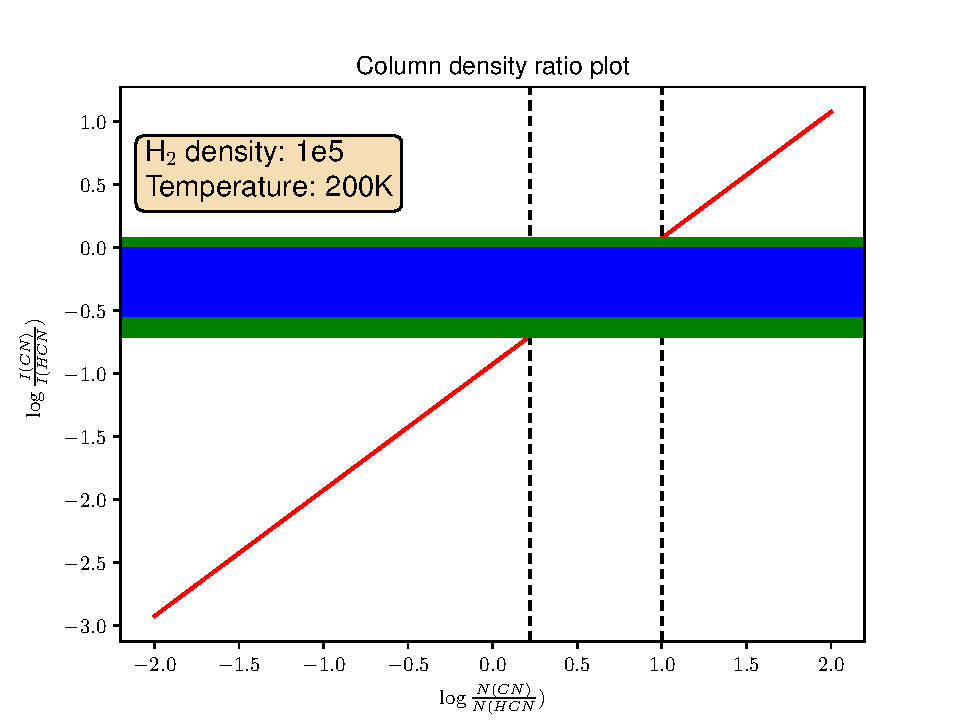
\includegraphics[width=10cm]{Nratios_plot_nH2-1e5_200K.eps}
      \caption{CN/HCN column density ratio for hydrogen densities of $n_\mathrm{H_2} = 10^5$ cm$^{-3}$ and kinetic temperatures of $T_\mathrm{kin} = 200$ K (red line). The observed line intensity ratio is plotted in blue (protostars positions) and green (all positions).}
         \label{1e5_75K}
\end{figure}

Column densities can be independently determined using molecular excitation models. Line ratio can provide additional information concerning physical properties of the observed gas. 

The non-LTE radiative transfer code RADEX (\citealt{vdT07}) was run in order to prepare sets of molecular excitation models. The CN and HCN molecules column density ratio, hydrogen number density and kinetic temperature of the gas were free parameters. HCN column density was chosen as 10$^8$ cm$^{-2}$ in order to ensure optically thin emission. CN column density parameter varies from 10$^6$ cm$^{-2}$ to 10$^{10}$ cm$^{-2}$ what translates into $N_\mathrm{CN}$/$N_\mathrm{HCN}$ in following limits: 10$^{-2}$-10$^{2}$. The sets of models were obtained assuming a line width of 1.0 km s$^{-1}$, hydrogen densities of $n_\mathrm{H_2} = 10^3$ cm$^{-3}$, $n_\mathrm{H_2} = 10^4$ cm$^{-3}$ and $n_\mathrm{H_2} = 10^5$ cm$^{-3}$ and kinetic temperatures of $T_\mathrm{kin} = 30$ K, $T_\mathrm{kin} = 75$ K and $T_\mathrm{kin} =200$ K. The molecular data files used during modelling were procured from the Leiden Atomic and Molecular Database (LAMDA, \citealt{Sch05}).

Fig.~\ref{1e5_75K} presents one exemplary set of models of CN/HCN column density ratio versus the modelled line intensities ratio for hydrogen densities of $n_\mathrm{H_2} = 10^5$ cm$^{-3}$ and kinetic temperatures of $T_\mathrm{kin} = 200$ K. The rest of the models are shown in the Appendix B. CN/HCN column density ratio weakly depends on hydrogen density and kinetic temperature in the low limit of those parameters. All presented models show similar properties.

The modelled line intensities are compared with the observations. The observed line intensity ratio covers a range of \mbox{0.0-1.0} of the column density ratio in the logarithmic scale. That corresponds to a few times higher CN column density than the same parameter of HCN. This result slightly depends on hydrogen densities and kinetic temperature of the gas (see Table~\ref{table:5}).

\begin{table}
\caption{CN/HCN column density ratio}             % title of Table
\label{table:5}      % is used to refer this table in the text
\centering                          % used for centering table
\begin{tabular}{c c c} 
\hline\hline  
$n_\mathrm{H_2}$ & $T_\mathrm{kin}$ & log$_{10}$(N[CN]/N[HCN]) \\
$($cm$^{-3})$ & (K) & \\
\hline
10$^{3}$ & 30 & 0.03-0.88\\
10$^{3}$ & 75 & 0.06-0.84\\
10$^{3}$ & 200 & 0.00-0.78\\ \hdashline
10$^{4}$ & 30 & 0.16-0.94\\
10$^{4}$ & 75 & 0.08-0.86\\
10$^{4}$ & 200 & 0.04-0.82\\ \hdashline
10$^{5}$ & 30 & 0.20-0.98\\
10$^{5}$ & 75 & 0.18-0.86\\
10$^{5}$ & 200 & 0.22-1.00\\ \hline
\end{tabular}
\end{table} 

%The sets of models shown in this section indicate that CN/HCN column density ratio covers the range of 1-10 regardless of excitation conditions. This result suggests that the UV radiation may play an important role around low-mass protostars. 

\section{Discussion}

\subsection{Astrochemical model}

In Section 3.2 we have raised a question about influence of the UV radiation on the surrounding of the observed sources. We used the Nahoon astrochemical model in order to estimate the intensity of the UV field in reference to units of the interstellar UV field $G_0$.

The Nahoon is a numerical code allowing to determine the gas-phase chemistry in astrononomical context  (\citealt{Wak12}). The solver computes the chemical evolution in time of 489 species involving 6992 gas-phase and gas-grain reactions based on rate coefficients stored in the Kinetic Database for Astrochemistry (KIDA)\footnote{http://kida.obs.u-bordeaux1.fr/}. The Nahoon code can model chemistry at a fixed temperature and density (0D modeling), as well as at grid of temperature, density and visual extinction (1D modeling). The UV radiation is described through the relation between visual extinction $A_\mathrm{V}$ and the photodissociation rate coefficient $k$ Eq~\ref{eq3}:
\begin{equation} \label{eq3}
k = \alpha e^{-\gamma A_\mathrm{V}}
\end{equation}
Here, $\mathrm{\alpha}$ and $\mathrm{\gamma}$ are coefficients of photodissociation HCN equal $1.64\times10^{-9}$ and $3.12$ respectively (\cite{Hea17}). 
All models were performed at the 1D modeling grid with the latest version of the Nahoon code (Nahoon\_kida.uva.2014).


\begin{figure}
\centering
\includegraphics[width=10cm]{starless.eps}
\caption{Time evolution of CN (red line), HCN (blue line) and CS (black line) abundances obtained with Nohoon astrochemical code with initial parameters of $n_\mathrm{HI+2 \dot H_2} = 10^4$ cm$^{-3}$, $T = 10$ K, $A_\mathrm{V}$ = 5 mag. The assumed cosmic-ray ionization rate is $1.3\times10^{17}$ s$^{-1}$, dust to gas mass ratio is 0.01, dust grain radius is $10^{-5}$ cm, grain density is 3 g cm$^{-3}$.}
\label{starless}
\end{figure}

The evolution of the chemical network was started at the time of a dense cloud formation. Figure~\ref{starless} shows a model corresponding to a typical dense cloud with temperature of 10 K and hydrogen total density of $n_\mathrm{HI+2 \dot H_2} = 10^4$ cm$^{-3}$. The chemical composition of the CN, HCN and CS molecules stabilises at the time of $10^{7}$ yrs with HCN abundance higher with respect to CN. We assumed the time of $10^{6}$ yrs as the time when the star formation starts in dense clouds. The modelled abundances of the all 474 species at the time of $10^{6}$ yrs were used as an input data for the following set of models.

\begin{figure}
\centering
\includegraphics[width=10cm]{G0.eps}
\caption{Similar to Fig.~\ref{AV5} but for fixed temperature $T = 50$ K.}
\label{G0}
\end{figure}


The closest neighbourhood of low-mass protostars was simulated, based on the initial abundances of all species from starless cloud modelling. We adopted the UV radiation and cosmic ray fluxes typical for dense clouds as an initial conditions. The visual extinction and the total cosmic-ray ionization rate were set as 5 mag and $1.3\times 10^{17}$ s$^{-1}$ respectively. The sets of models were run for the temperature range between 10 and 200 K and the total hydrogen densities from $10^4$ cm$^{-3}$ to $10^6$ cm$^{-3}$. The results (Fig.~\ref{AV5}) are consistent with starless cloud model. Without any additional source of the UV radiation HCN is more abundant than CN about 2-3 orders of magnitude. Moreover, the model shows that CN/HCN abundances ratio is slightly dependent on gas temperature up to 150 K. 

This results justify assumptions for the modelling the neighbourhood of low-mass protostars with the fixed gas temperature of 50 K. The code was run for the range of visual extinction between $-4.5^{\mathrm{m}}$ and $2.5^{\mathrm{m}}$ what corresponds to the UV radiation field G$_0$ of $4\times 10^{-4}$ to $1.25\times 10^{6}$. The computed CN/HCN abundances ratio is presented in Fig.~\ref{G0}. The calculated column density ratio covers parameter space of all probed densities and G$_0$ range between $10^{-4}$ and 0.05 in weak UV radiation regime. The observed CN/HCN ratio is reproduced at the G$_0$ values greater than $1.5 \times 10^{3}$ as well. HCN is more abundant than CN in very weak (<$10^{3}$ G$_0$) radiation field. This result is consistent with simulations of a starless cloud what leads to conclusion that additional UV radiation source is needed to reproduce the observational ratios. 

Comparing CN/HCN results with similar plots of CN/CS and CS/HCN ratio (Fig.~\ref{CN/CS} and Fig.~\ref{CS/HCN} respectively) restricts the parameter space to very low-density and weakly irradiated gas or dense gas with strong UV radiation. CN/CS ratio varies between 9 and 29 for the all protostars positions, while CS/HCN ratio is in order of 0.12-0.26. Astrochemical models computed for these molecules show similar behaviour as that presented for CN/HCN ratio. UV radiation with the strength of G$_0$ in order of $10^{3}-10^{4}$ is not very probable in low-mass protostars neighbourhood. At the protostars positions high hydrogen densities can be assumed. Astronomical models show that an additional UV radiation source of the strength of few hundredth of the average interstellar UV radiation field is required to cover the observational ratios.

Low CN/HCN ratio found in astrochemical model for strongly irradiated gas was a surprising result. Both production and destruction of each molecule need to be investigated in order to explain what is the reason of higher HCN abundances than expected. Detailed models of the most dominant reactions for destruction and production of each molecule are presented in Fig. ~\ref{CN_dest} – Fig.~\ref{HCN_prod} with the assumption of fixed 50 K temperature. Reaction flux is defined as reactants abundances multiplied by reaction rate coefficient. Only these reactions were taken into consideration which accumulated flux is greater than 80$\%$ of the total flux of all reactions contributed in the studied molecules destruction or production processes. 

The reactions distribution in the parameter space is not very strongly depended on hydrogen densities. The strength of an additional UV radiation source is the parameter that distinguishes the dominant reactions the most. It was divided into three regimes: with weak, intermediate and strong UV field. The reactions which contamination in CN or HCN production or destruction is greater than 30$\%$ are listed in Tab.~\ref{reactions} as well as illustrated in Fig.~\ref{reactions_smallG0}- Fig.~\ref{reactions_largeG0}.

In the regime of weak UV radiation fields dominant formation channels of CN and HCN are hydrocarbons (CH and CH$_2$ respectively) reactions with atomic nitrogen. In more dense areas electronic reaction with CNC cation plays role in the CN formation. The destruction of CN is mostly dominated by reaction with neutral oxygen (60-70$\%$) or nitrogen (30$\%$ or less). In weakly irradiated environment atomic elements are more abundant in the neutral state. More ionised atoms are produced with increasing the UV radiation what blocks these effective channels of CN destruction. 

On the other hand, HCN destruction is driven by many channels in the weakest UV regime. Simultaneous impact of few different reactions is not that effective as the reaction ruling the CN destruction. It leads to higher HCN abundances in respect to CN. For slightly stronger radiation fields in order of $10^{-3}$ HCN reaction with abundant C+ is the dominant destructive reaction. This reaction results in CNC+ production what quickly reacts with electron forming CN. That explains why CN/HCN ratio increases with larger radiation. 

CN/HCN ratio is widely used as UV radiation tracer in PDRs (eg. \citealt{Thi04}, \citealt{Han15}). HCN photodissociates into CN molecule and H atom, while CN requires more energetic photon (> 12.4 eV) to be disintegrated (\citealt{vDi87}). This leads to higher abundance of CN molecules and increases CN/HCN column density ratio. Fluxes of HCN photodissociation (Fig.~\ref{HCN_dest}) show that this reaction has marginal contribution in nitrogen chemistry up to G$_0$ $\approx$ 100.


\begin{table*}
\caption{Dominant processes in CN, HCN chemistry}             % title of Table
\label{reactions}      % is used to refer this table in the text
\centering                          % used for centering table
\begin{tabular}{c c c c} 
\hline\hline  
Molecule & Weak UV fields  & Medium UV fields  & Strong UV fields  \\
& (G$_0$ = $10^{-3} - 10^{-1})$ & (G$_0$ = $10^{-1} - 10^{1})$ & (G$_0$ = $10^{1} - 10^{6})$ \\
\hline
\multirow{8}{*}{CN} & \multicolumn{3}{c}{\textbf{Destruction}}\\
&O + CN $\rightarrow$ N + CO & CN + ph $\rightarrow$ C + N & CN + ph $\rightarrow$ C + N\\
&CN + N $\rightarrow$ C + N$_2$ & O + CN $\rightarrow$ N + CO & \\ \vspace{2.5 pt}
&\multicolumn{3}{c}{\textbf{Production}}\\
&N + CH $\rightarrow$ H + CN & N + C$_2$ $\rightarrow$ C + CN &  HCN$^+$ + e$^-$ $\rightarrow$ H + CN\\
&CNC$^+$ + e$^-$ $\rightarrow$ C + CN & H + CN$^+$ $\rightarrow$ CN + H$^+$ & N + CH $\rightarrow$ H + CN\\ 
&N + C$_2$ $\rightarrow$ C + CN &  & H + CN$^+$ $\rightarrow$ CN + H$^+$\\
&  &   & N + C$_2$ $\rightarrow$ C + CN\\ \hline
\multirow{9}{*}{HCN} & \multicolumn{3}{c}{\textbf{Destruction}}\\
&HCN + C$^+$ $\rightarrow$ H + CNC$^+$ & HCN + C$^+$ $\rightarrow$ H + CNC$^+$ &  HCN + ph $\rightarrow$ H + CN\\
&HCN$^+$ + HCO$^+$ $\rightarrow$ CO + HCNH$^+$ &HCN + ph $\rightarrow$ H + CN & HCN + C$^+$ $\rightarrow$ H + CNC$^+$\\ 
&HCN + H$^+$ $\rightarrow$ H + HNC$^+$ &  &  \\
&HCN + ph $\rightarrow$ H + CN &  &  \\ \vspace{2.5 pt}
&\multicolumn{3}{c}{\textbf{Production}}\\
&N + CH$_2$ $\rightarrow$ H + HCN & H + CCN $\rightarrow$ C + HCN & HCNH$^+$ + e$^-$ $\rightarrow$ H + HCN\\
&H + CCN $\rightarrow$ C + HCN & HCNH$^+$ + e$^-$ $\rightarrow$ H + HCN & H + CCN $\rightarrow$ C + HCN\\
&HCNH$^+$ + e$^-$ $\rightarrow$ H + HCN & & \\
&C + HNC $\rightarrow$ C + HCN & & \\ \hline
\end{tabular}
\end{table*} 



\section{Conclusions}

\begin{itemize}
\item HCN $J=1-0$ and CN $J=1-0$ show different spatial distribution. The emission of CN is concentrated at the positions of protostars, while HCN traces molecular outflows. 
\item CN/HCN column density ratio is in the range of 1-10 calculated both with LTE and non-LTE assumption.
\item An additional source of UV radiation of the strength G$_0$ $\approx$ $10^{-2}$ is required to cover the observational CN/HCN range. There is non-zero UV radiation field around low-mass protostars.
\item CN/HCN ratio starts to play important role in the nitrogen bearing spieces chemistry at G$_0$ $\approx$ $10^{2}$.
\end{itemize}



\begin{acknowledgements}
AM, AK and MG are supported by the Polish National Science Center grants NAVA InterAPS and 2016/21/D/ST9/01098. 

This research has made use of data from the Herschel Gould Belt survey (HGBS) project (http://gouldbelt-herschel.cea.fr). The HGBS is a Herschel Key Programme jointly carried out by SPIRE Specialist Astronomy Group 3 (SAG 3), scientists of several institutes in the PACS Consortium (CEA Saclay, INAF-IFSI Rome and INAF-Arcetri, KU Leuven, MPIA Heidelberg), and scientists of the Herschel Science Center (HSC).
\end{acknowledgements}


% WARNING
%-------------------------------------------------------------------
% Please note that we have included the references to the file aa.dem in
% order to compile it, but we ask you to:
%
% - use BibTeX with the regular commands:
\bibliographystyle{aa} % style aa.bst
\bibliography{amirocha} % your references Yourfile.bib
%
% - join the .bib files when you upload your source files
%-------------------------------------------------------------------

\begin{appendix} %First appendix
\section{Spectral Energy Distributions}

Broad-band observations are needed in order to determine physical properties of a protostar. Dunham et al. 2015 studied properties of protostars in the Serpens molecular cloud using 2MASS (\citealt{Skr06}) and Spitzer IRAC/MIPS (\citealt{Eva09}), observations covering the range of 1.25–70 $\mu$m, photometry from Wide-field Infrared Survey Explorer 12 and 22 $\mu$m (WISE; \citealt{Wri10}), SHARC-II 350 $\mu$m (\citealt{Sur16}), the SCUBA Legacy Catalog 450 and 850 $\mu$m (\citealt{dFr08}) and 1.1 mm observations from Bolocam dust survey (\citealt{Eno07}). The Serpens Main region was also observed during the Herschel Gould Belt survey project (\citealt{And10}). SPIRE/PACS photometry in the Serpens molecular cloud is discussed in Fiorellino et al. (in prep.). 

Based on SEDs the bolometric temperature and luminosity can be calculated for each of the observed protostars. The bolometric luminosity was determined by integrating the SEDs over frequency:
\begin{equation} \label{eq1}
L_{bol} = \pi \, d^2 \, \int F_\nu d\nu
\end{equation}
where $d$ is the cloud distance of $436 \pm 9.2$ pc (\citealt{Ort17}).
The bolometric temperature was calculating as described in \citealt{Mye93}:
\begin{equation} \label{eq2}
T_{bol} = 1.25 \, 10^{-11} \, \bar{\nu}
\end{equation}
where $\bar{\nu}$ is the mean frequency given by:
\begin{equation} \label{eq3}
\bar{\nu} = \frac{\int \nu F_\nu d\nu}{ \int F_\nu d\nu}
\end{equation}

Using Scipy \textit{splrep} and \textit{splev} functions cubic smooth spline interpolation of the photometric data was performed while calculating the protostars parameters. Integration along the resulting axis was obtain with the composite trapezoidal rule (\textit{Scipy} package). The photometric data allows us to perform the integration along wide range of wavelength with exception of SMM8. Here we have only 4 photometric points from the Herschel Gould Belt so the calculeted bolometric luminosity and temperature can be underestimated.


\begin{figure}
   \includegraphics[width=8cm]{serpens_seds.eps}
      \caption{Spectral Energy Distributions of protostars in the Serpens Main region.}
         \label{seds}
   \end{figure}


\section{Astrochemical models}

\begin{figure}
\centering
\includegraphics[width=10cm]{AV5.eps}
\caption{Contour plot of Nahoon sets of models of CN/HCN abundances ratio with fixed visual extinction $A_\mathrm{V}$ = 5 mag at the time of 10$^{7}$ yrs after star formation began in the cloud.} 
\label{AV5}
\end{figure}

\begin{figure}
   \centering
   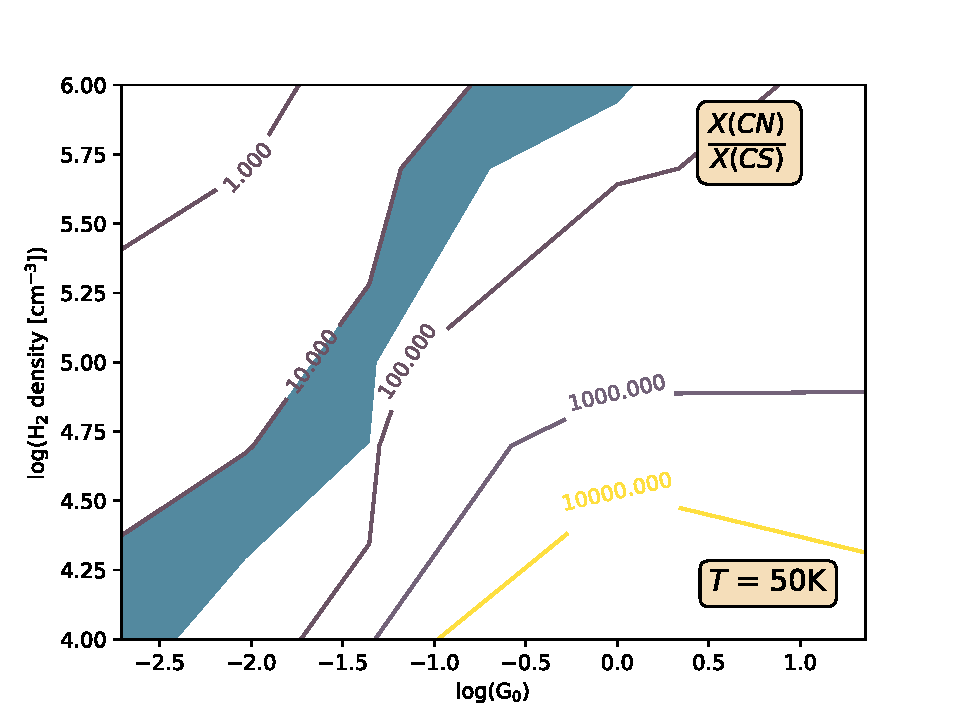
\includegraphics[width=10cm]{CN_CS.eps}
      \caption{Similar to Fig.~\ref{G0} but for CN/CS ratio.}
         \label{CN/CS}
   \end{figure}

\begin{figure}
   \centering
   \includegraphics[width=10cm]{CS_HCN.eps}
      \caption{Similar to Fig.~\ref{G0} but for CS/HCN ratio.}
         \label{CS/HCN}
   \end{figure}

\section{Dominant reactions in CN, HCN chemistry}

\begin{figure}
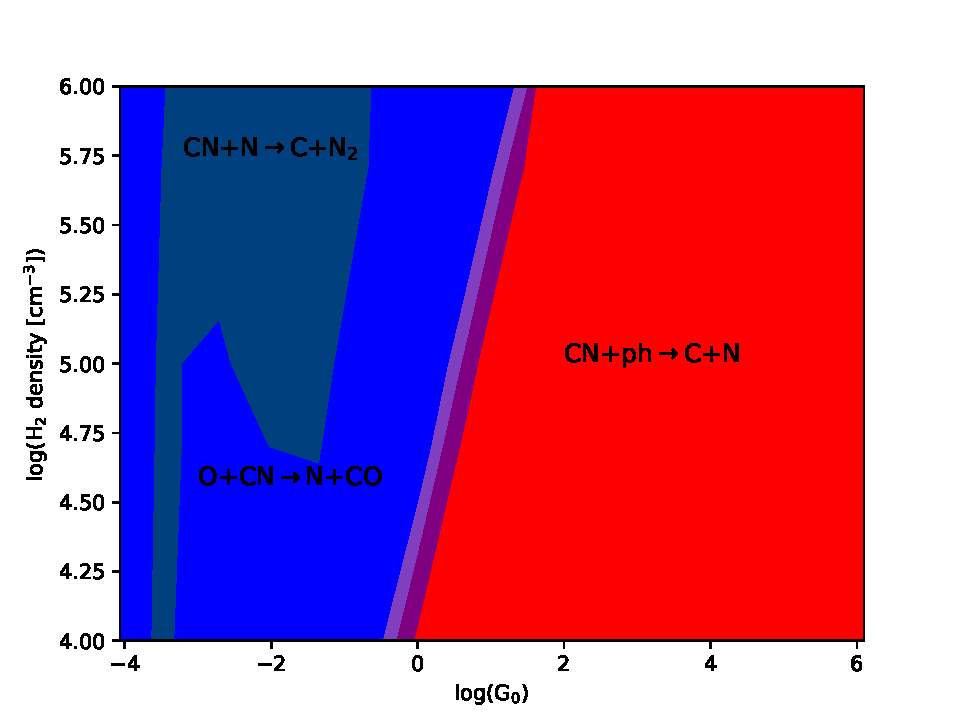
\includegraphics[width=10cm]{destruction_CN_dominant.eps}
\caption{Dominant reactions of CN destruction. Reactions conributed at least 50$\%$ of total flux are marked with full colous. Transparent colours correspond to 30$\%$-50$\%$ contribution.}
\label{CN_dest}
\end{figure}

\begin{figure}
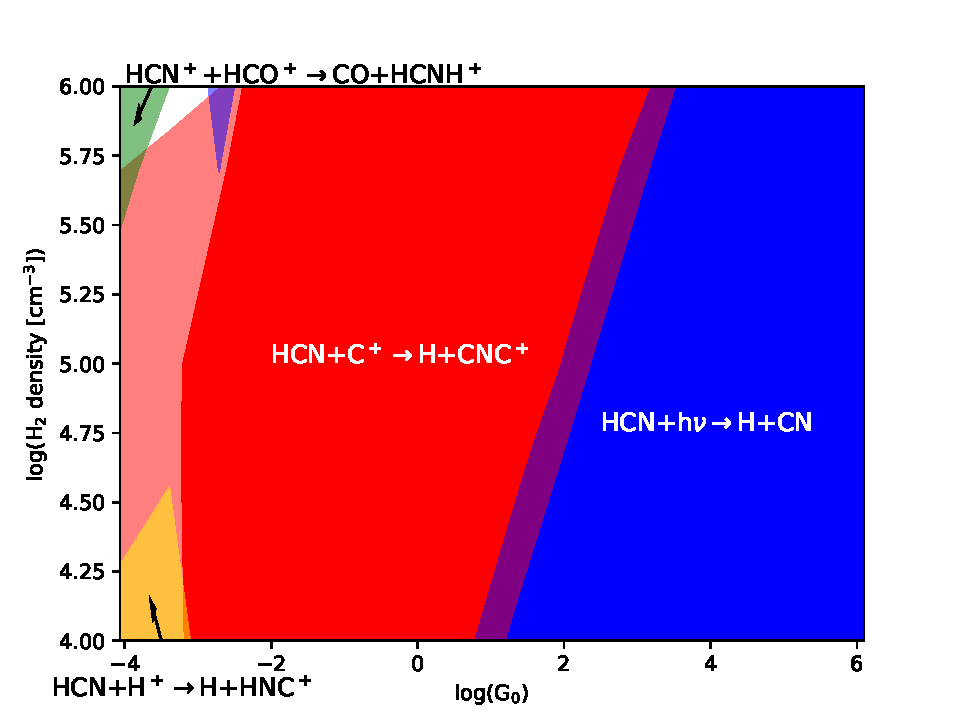
\includegraphics[width=10cm]{destruction_HCN_dominant.eps}
\caption{Similar to Fig.~\ref{CN_dest} but for HCN destruction.}
\label{HCN_dest}
\end{figure}

\begin{figure}
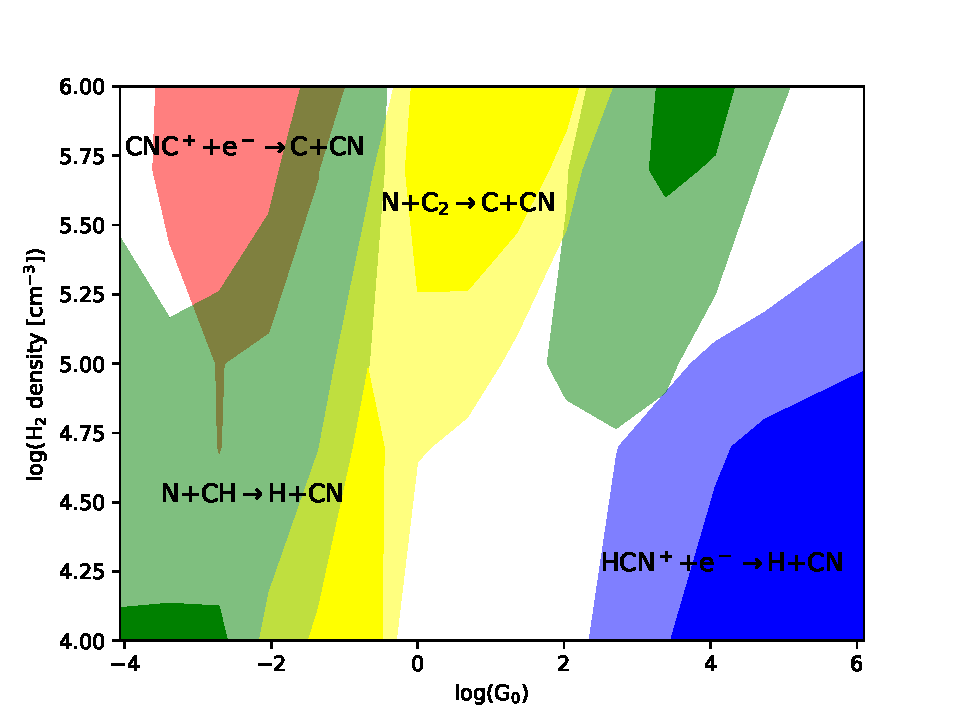
\includegraphics[width=10cm]{production_CN_dominant.eps}
\caption{Similar to Fig.~\ref{CN_dest} but for CN production.}
\label{CN_prod}
\end{figure}

\begin{figure}
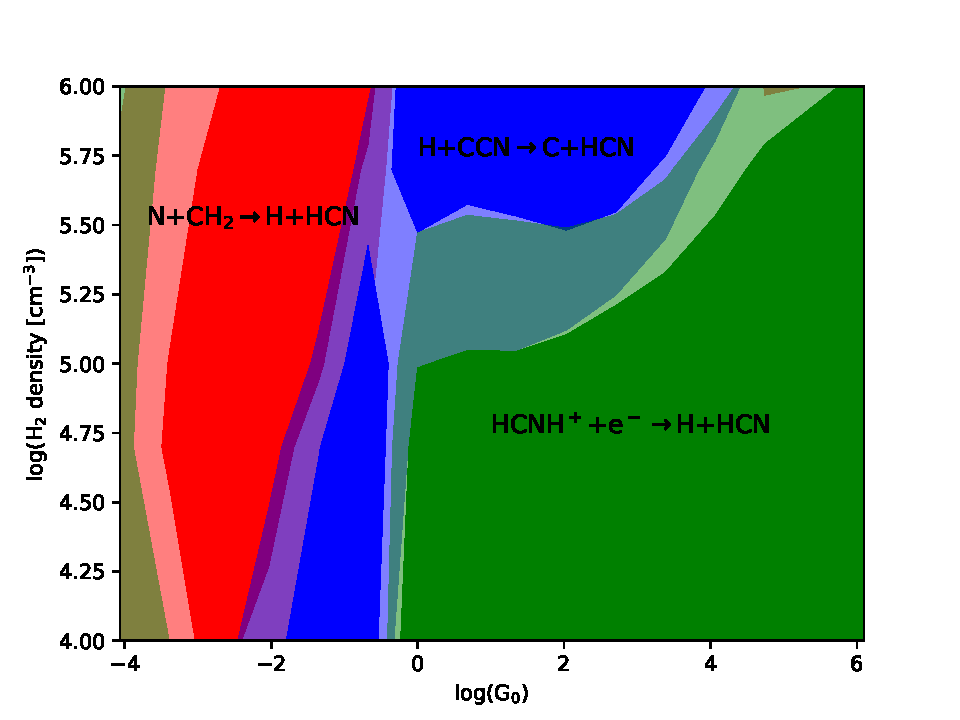
\includegraphics[width=10cm]{production_HCN_dominant.eps}
\caption{Similar to Fig.~\ref{CN_dest} but for HCN production.}
\label{HCN_prod}
\end{figure}

\begin{figure}
\includegraphics[width=10cm]{reactions-smallG0.eps}
\caption{Reactions network for weakly UV irradiated gas.}
\label{reactions_smallG0}
\end{figure}

\begin{figure}
\includegraphics[width=10cm]{reactions-mediumG0.eps}
\caption{Similar to Fig.~\ref{reactions_smallG0} but for UV field of G$_0$ = $10^{-1} - 10^{1})$.}
\label{reactions_mediumG0}
\end{figure}

\begin{figure}
\includegraphics[width=10cm]{reations_large.eps}
\caption{Similar to Fig.~\ref{reactions_smallG0} but for for UV field higher than G$_0$ = $10^{1})$.}
\label{reactions_largeG0}
\end{figure}

\section{Tables}
\begin{table*}
\caption{Integrated fluxes of the observed line at the positions of protostars}             % title of Table
\label{table:fluxes}      % is used to refer this table in the text
\centering                          % used for centering table
\begin{tabular}{l l c c c c} 
\hline\hline 
Source & Line & $\int{T_{mb} \, dV}$ & T$_\mathrm{peak}$ & N$_\mathrm{up}$ & N$_\mathrm{tot}$\\
 &  & (K km/s) & (K) & (cm$^{-2}$) & (cm$^{-2}$) \\
\hline  
\multirow{5}{*}{SMM1} & CN 1-0 & 5.26 & 0.89 & 1.1$\times$10$^{13}$ & 6.6$\times$10$^{14}$\\
{} & HCN 1-0 & 8.23 & 1.76 & 5.2$\times$10$^{12}$ & 2.0$\times$10$^{14}$\\ 
{} & CS 3-2 & 2.98 & 1.57 & 2.1$\times$10$^{12}$ & 2.3$\times$10$^{13}$\\  
{} & C$^{34}$S 3-2 & 1.21 & 0.56 &  & \\ 
{} & H$^{13}$CN 1-0 & 1.43 & 0.45 &  & \\ 
\hline
\multirow{5}{*}{SMM2} & CN 1-0 & 8.41 & 1.92 & 1.8$\times$10$^{13}$ & 1.1$\times$10$^{15}$ \\
{} & HCN 1-0 & 12.57 & 3.48 & 8.0$\times$10$^{12}$ & 3.0$\times$10$^{14}$\\ 
{} & CS 3-2 & 6.57 & 3.10 & 4.5$\times$10$^{12}$ & 2.0$\times$10$^{13}$\\  
{} & C$^{34}$S 3-2 & 0.89 & 0.47 & &\\
{} & H$^{13}$CN 1-0 & 1.65 & 0.64 &  & \\ 
\hline
\multirow{5}{*}{SMM3} & CN 1-0 & 13.18 & 3.42 & 2.8$\times$10$^{13}$ & 1.7$\times$10$^{15}$\\
{} & HCN 1-0 & 14.14 & 4.95 & 8.9$\times$10$^{12}$ & 3.4$\times$10$^{14}$\\ 
{} & CS 3-2 & 8.11 & 2.90 & 5.6$\times$10$^{13}$ & 6.2$\times$10$^{13}$ \\  
{} & C$^{34}$S 3-2 & 0.604 & 0.36 &  & \\
{} & H$^{13}$CN 1-0 & 0.88 & 0.41 &  & \\ 
\hline
\multirow{5}{*}{SMM4} & CN 1-0 & 9.89 & 1.90 & 2.1$\times$10$^{13}$ & 1.3$\times$10$^{15}$\\
{} & HCN 1-0 & 17.59 & 4.69 & 1.1$\times$10$^{13}$ & 4.2$\times$10$^{14}$\\ 
{} & CS 3-2 & 14.4 & 4.30 & 9.9$\times$10$^{12}$ & 1.1$\times$10$^{14}$\\  
{} & C$^{34}$S 3-2 & 1.56 & 0.64 & &\\ 
{} & H$^{13}$CN 1-0 & 1.83 & 0.61 & &\\ 
\hline
\multirow{5}{*}{SMM5} & CN 1-0 & 3.49 & 0.94 & 7.3$\times$10$^{12}$ & 4.4$\times$10$^{14}$\\
{} & HCN 1-0 & 5.79 & 1.72 & 3.7$\times$10$^{12}$ & 1.4$\times$10$^{14}$\\ 
{} & CS 3-2 & 2.61 & 1.48 & 1.8$\times$10$^{12}$ & 2.0$\times$10$^{13}$\\  
{} & C$^{34}$S 3-2 & 0.28 & 0.42  &  & \\ 
{} & H$^{13}$CN 1-0 & 1.16 & 0.42  & & \\ 
\hline
\multirow{5}{*}{SMM6} & CN 1-0 & 10.57 & 3.17 & 2.2$\times$10$^{13}$ & 1.3$\times$10$^{15}$\\
{} & HCN 1-0 & 11.85 & 5.15 & 8.9$\times$10$^{12}$ & 3.3$\times$10$^{14}$\\ 
{} & CS 3-2 & 7.86 & 3.2 & 5.4$\times$10$^{12}$ & 6.0$\times$10$^{13}$\\  
{} & C$^{34}$S 3-2 & 0.74 & 0.56 & & \\ 
{} & H$^{13}$CN 1-0 & 0.81 & 0.40 & & \\
\hline
\multirow{5}{*}{SMM8} & CN 1-0 & 5.09 & 0.94 & 1.1$\times$10$^{13}$ & 6.4$\times$10$^{14}$\\
{} & HCN 1-0 & 6.32 & 1.72 & 4.0$\times$10$^{12}$ & 1.5$\times$10$^{14}$ \\ 
{} & CS 3-2 & 4.64 & 2.08 & 3.2$\times$10$^{12}$ & 3.5$\times$10$^{13}$ \\  
{} & C$^{34}$S 3-2 & 0.22 & 0.35 &  &  \\ 
{} & H$^{13}$CN 1-0 & 0.46 & 0.21 &  & \\
\hline
\multirow{5}{*}{SMM9} & CN 1-0 & 5.41 & 0.84 & 1.1$\times$10$^{13}$ & 6.8$\times$10$^{14}$\\
{} & HCN 1-0 & 14.08 & 2.40 & 8.9$\times$10$^{12}$ & 3.4$\times$10$^{14}$ \\ 
{} & CS 3-2 & 9.85 & 2.70 & 6.8$\times$10$^{12}$ & 7.5$\times$10$^{13}$\\ 
{} & C$^{34}$S 3-2 & 1.3 & 0.62 &  & \\ 
{} & H$^{13}$CN 1-0 & 1.57 & 0.38 & & \\ 
\hline
\multirow{5}{*}{SMM10} & CN 1-0 & 2.59 & 0.78 & 5.4$\times$10$^{12}$ & 3.3$\times$10$^{14}$\\
{} & HCN 1-0 & 6.96 & 1.75 & 4.4$\times$10$^{12}$ & 1.7$\times$10$^{14}$\\ 
{} & CS 3-2 & 3.83 & 1.43 & 2.6$\times$10$^{12}$ & 2.9$\times$10$^{13}$ \\  
{} & C$^{34}$S 3-2 & 0.56 & 0.40 &  & \\ 
{} & H$^{13}$CN 1-0 & 0.98 & 0.45 &  &\\ 
\hline
\multirow{5}{*}{SMM12} & CN 1-0 & 9.10 & 1.85 & 1.9$\times$10$^{13}$ & 1.2$\times$10$^{15}$\\
{} & HCN 1-0 & 13.27 & 3.50 & 8.4$\times$10$^{12}$ & 3.2$\times$10$^{14}$\\ 
{} & CS 3-2 & 9.75 & 3.26 & 6.7$\times$10$^{12}$ & 7.4$\times$10$^{13}$\\  
{} & C$^{34}$S 3-2 & 1.18 & 0.58 &  &\\ 
{} & H$^{13}$CN 1-0 & 1.43 & 0.46 & & \\ 
\hline
\end{tabular}
\end{table*}

\end{appendix}

\end{document}
%
%%%%%%%%%%%%%%%%%%%%%%%%%%%%%%%%%%%%%%%%%%%%%%%%%%%%%%%%%%%%%%
Example below of non-structurated natbib references  
To use the v8.3 macros with this form of composition of bibliography, 
the option "bibyear" should be added to the command line 
"\documentclass[bibyear]{aa}".
%%%%%%%%%%%%%%%%%%%%%%%%%%%%%%%%%%%%%%%%%%%%%%%%%%%%%%%%%%%%%%




